\documentclass[English,t,% 't' (resp. 'c') places text vertically at top/center of the slides
% PDF settings
hyperref={%
    pdftitle={FISA-DE2 OOP in Java},%
    pdfauthor={Guillaume Muller},%
    pdfsubject={OOP in Java},%
    pdfkeywords={OOP,Java}%
    },%
% To load many pre-defined color names
xcolor={pdftex,svgnames} % dvipsnames, dvipsnames*, svgnames, svgnames*, x11names,
]{beamer}
\usetheme{Copenhagen} % AnnArbor,Antibes,Bergen,Berkeley,Berlin,Boadilla,CambridgeUS,Copenhagen,Darmstadt,Dresden,Frankfurt,Goettingen,Hannover,Ilmenau,JuanLesPins,Luebeck,Madrid,Malmoe,Marburg,Montpellier,PaloAlto,Pittsburgh,Rochester,Singapore,Szeged,Warsaw,boxes,default

% Correct French/English indentation and splitting of words
\usepackage{babel}

% Correct management of accentuated chars in input file
\usepackage[utf8]{inputenc}
%\usepackage[utf8]{inputenc}

% Correct font for the generation of docs with accentuated chars
\usepackage[T1]{fontenc}      % Can handle hyphenation of words with accented characters
%%\usepackage[OT1]{fontenc}   % Might generated bad looking PDFs

% Access to many maths symbols
\usepackage{amsthm}
\usepackage{amsmath}
\usepackage{amsfonts}

% Insertion of images generated by external tools
\usepackage{graphicx}

% To generate pretty & scalable images directly in LaTeX
\usepackage{tikz}
% \draw[decorate,decoration={coil,amplitude=1.5cm, segment length=.4cm}] (5,5.5) -- (5,1.5) ;
\usetikzlibrary{tikzmark}
\usetikzlibrary{calc}
\usetikzlibrary{decorations.text}
\usetikzlibrary{decorations.shapes}
\usetikzlibrary{decorations.pathmorphing,snakes}

\def\me{Guillaume \textsc{Muller}}

% To print numbers correctly
\usepackage{numprint}

% To position text blocks absolutely
\usepackage[absolute,overlay]{textpos}

% For UML diagrams
\usepackage{tikz-uml}

% To be able to strikeout text
\usepackage[normalem]{ulem}

% To be able to insert code listing
\usepackage{listings}

\definecolor{dkgreen}{rgb}{0,0.6,0}
\definecolor{gray}{rgb}{0.5,0.5,0.5}
\definecolor{mauve}{rgb}{0.58,0,0.82}

\lstset{frame=none,
  language=Java,
  aboveskip=1mm,
  belowskip=1mm,
  showstringspaces=false,
  columns=flexible,
  basicstyle={\tiny \ttfamily},
  numbers=left,
  numberstyle=\tiny\color{gray},
  keywordstyle=\color{blue},
  commentstyle=\color{dkgreen},
  stringstyle=\color{mauve},
  breaklines=true,
  breakatwhitespace=true,
  tabsize=2
}

% Info for title page
\title[OOP in Java]{Object-Oriented Programming in Java}
\logo{
\includegraphics[width=1cm]{images00/logo_tse.png}}
\author[\me{}]{\me{}}
\institute[TSÉ + LHC]{
  \inst{Telecom Saint-Étienne, Laboratoire Hubert-Curien}%
}
\date[09/14/2020]{14~September~2020}
\subject{OOP in Java}


%%%%%%%%%%%%%%%%%%%%%%%%%%%%%%%%%%%%%%%%%%%%%%%%%%%%%%%%%%%%%%%%%%%%%%
\begin{document}

% The title page
\begin{frame}
  \titlepage
\end{frame}

% %%%%%%%%%%%%%%%%%%%%%%%%%%%%%%%%%%%%%%%%%%%%%%%%%%%%%%%%%%%%%%%%%%%%%%
% % The TOC
% \begin{frame}{Table of contents}
%   \tableofcontents
% \end{frame}

%%%%%%%%%%%%%%%%%%%%%%%%%%%%%%%%%%%%%%%%%%%%%%%%%%%%%%%%%%%%%%%%%%%%%%
\begin{frame}{Object-Oriented Programming}

  \begin{itemize}
%
    \item Who knows what it is???
%
    \item Who has already used it???
%
    \item Who can cite it core principles???
%
    \item Who can cite a few languages using it???
%
  \end{itemize}

\end{frame}

%%%%%%%%%%%%%%%%%%%%%%%%%%%%%%%%%%%%%%%%%%%%%%%%%%%%%%%%%%%%%%%%%%%%%%
\begin{frame}{Programming Paradigms\footnote{Thought patterns/«~façons de voir le monde~».}- \onslide*<1>{Why~?}\onslide*<2>{How~?}}

  \onslide*<1>{
    \begin{itemize}
      \vspace{2em}
      \item Why do we need paradigms?
      \vspace{2em}
      \item Complex System $\Rightarrow$ ``Divide and Conquer''
      \vspace{2em}
      \item \textbf{Partitioning} the problem $\Rightarrow$ simpler discrete pieces
      \vspace{2em}
      \item Create \textbf{interfaces} \& \textbf{interactions} between these pieces
    \end{itemize}
  }

  \onslide*<2->{
  \begin{itemize}
    \item<2-> \textbf{Declarative} (what to execute $\Rightarrow$ goal to achieve)
    \begin{itemize}
      \item \textit{SQL, Prolog}
    \end{itemize}
%
    \item<3-> \textbf{Imperative} (how to execute $\Rightarrow$ explicit control flow)
    \begin{itemize}
      \item \textbf{Procedural}
      \begin{itemize}
        \item \textit{C, Pascal, Python, Lisp...}
      \end{itemize}
%
      \item \textbf{Functional}
      \begin{itemize}
        \item \textit{Caml, Haskell, Erlang, (Java)...}
      \end{itemize}
%
      \item \textcolor{blue}{\textbf{Object-Oriented}}
      \begin{itemize}
        \item \textit{\textcolor{blue}{Java}, C$\sharp{}$, (Python)...}
      \end{itemize}
%
    \end{itemize}
%
    \item<4-> \textbf{Event-Driven}
    \begin{itemize}
      \item \textit{Javascript, VisualBasic...}
    \end{itemize}
%
    \item<5-> \textbf{Reactive} (streams)
    \begin{itemize}
      \item \textit{(Java)...}
    \end{itemize}
%
  \end{itemize}
}

\end{frame}


%%%%%%%%%%%%%%%%%%%%%%%%%%%%%%%%%%%%%%%%%%%%%%%%%%%%%%%%%%%%%%%%%%%%%%
\begin{frame}{Objects \& Classes} % TODO: class attribute

\onslide*<1-6>{
  \begin{itemize}
    \item<2-6>{\textcolor{red}{Cars} of different types \tikzmark{Ca1}}
    \vspace{2em}
    \item<3-6>{\textcolor{green}{Clients} \tikzmark{Cl1}}
    \vspace{2em}
    \item<4-6>{\textcolor{blue}{Employees} (authorizations?) \tikzmark{E1}}
    \vspace{2em}
    \item<5-6>{\textcolor{black}{Contracts} \tikzmark{Co1}}
  \end{itemize}

  \begin{textblock*}{5cm}(10cm,5cm)%
    \begin{tikzpicture}[overlay,remember picture]
      \onslide*<1-6>{\node (label) at (0,0) {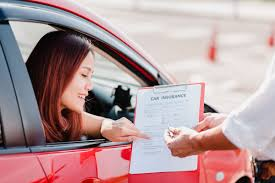
\includegraphics[width=5cm]{images02/car_rental.jpeg}};}
      % TODO: refaire avec des x/yshifts!!!
      \node (Ca2) at (-1.1,1.6) {};
      \node (Cl2) at (-.9,.5) {};
      \node (E2)  at (2.4,-.5) {};
      \node (Co2) at (.5,-1) {};

      \onslide*<2-6>{\draw[->, very thick, red]   (pic cs:Ca1) to (Ca2);}
      \onslide*<3-6>{\draw[->, very thick, green] (pic cs:Cl1) to (Cl2);}
      \onslide*<4-6>{\draw[->, very thick, blue]  (pic cs:E1)  to (E2);}
      \onslide*<5-6>{\draw[->, very thick, black] (pic cs:Co1) to (Co2);}
    \end{tikzpicture}
  \end{textblock*}
  \vspace{3em}
  \onslide*<6>{\center \huge \bf World = Set of typed objects}
}

\onslide*<7-10>{
  { \small
  \begin{itemize}
%
    \item<7-10> \textbf{Classes} = Object \textit{types/models} \\
    \vspace{.5em}
    \begin{itemize}
      \item Attributes (or Fields) \tikzmark{Attr1}\\
      = \textbf{Structure}
      \vspace{1em}
      \item Methods (\sout{"functions"})\tikzmark{Meth1}\\
      = \textbf{Behaviour}\\
      \onslide<9-10>{{\color{blue}\textit{constructors() = create instances}}}
      \item<8-10> {\small Attributes + Methods = «~\textbf{members}~»}
    \end{itemize}
%
    \vspace{2em}
    \item<10> \textbf{Objects} = \textit{valued instances}\\
%
  \end{itemize}
}

  \begin{textblock*}{3cm}(10cm,3cm)%
    \begin{tikzpicture}[overlay,remember picture]
      \node[xshift=-2cm,yshift=+.2cm] (Attr2) {};
      \node[xshift=-2cm,yshift=-1cm] (Meth2) {};
      \umlclass{Car}%
      {{\tiny \texttt{wheels: List<Wheel>}} \\ {\tiny \texttt{doors: List<Door>}}}
      {\onslide*<9-10>{\tiny \texttt{\color{blue}Car(\ldots{})}}\\{\tiny \texttt{drive()}}\\ {\tiny \texttt{changeWheel(newWheel: Wheel)}}}
      \draw[->, very thick] (pic cs:Attr1) to (Attr2);
      \draw[->, very thick] (pic cs:Meth1) to (Meth2);
    \end{tikzpicture}
  \end{textblock*}

  \onslide*<10>{
  \begin{textblock*}{3cm}(10cm,7cm)%
    \begin{tikzpicture}[overlay,remember picture]
      \umlclass{Jean's Car}%
      {{\tiny \texttt{wheels: \textcolor{red}{Jean's 4 wheels}}}\\ {\tiny \texttt{doors: \textcolor{red}{Jean's 3 doors}}}}
      {{\tiny \texttt{drive()}}\\ {\tiny \texttt{changeWheel(newWheel: Wheel)}}}
    \end{tikzpicture}
  \end{textblock*}
  }
}

\end{frame}


%%%%%%%%%%%%%%%%%%%%%%%%%%%%%%%%%%%%%%%%%%%%%%%%%%%%%%%%%%%%%%%%%%%%%%
\begin{frame}{Visibility \& Encapsulation}

  \begin{itemize}
%
    \item<1-> \textbf{\texttt{-} = private}\tikzmark{Priv1}
    \begin{itemize}
      \item same class
    \end{itemize}
%
    \item<1-> \textbf{\texttt{\#} = protected}\tikzmark{Prot1}
    \begin{itemize}
      \item same class, same package, derived
    \end{itemize}
%
    \item<1-> \textbf{\texttt{+} = public}\tikzmark{Pub1}
    \begin{itemize}
      \item everybody
    \end{itemize}
%
    \vspace{3em}
    \item<2> \textbf{Good practice} (SOLID, KISS, YAGNI, GRASP\ldots{})\footnote{cf. Wikipedia.}
    \begin{itemize}
      \item \textbf{private} for all Attributes
      \item public/protected \textbf{Accessors} (getXXX()/setXXX())
      \vspace{.5em}
      \item E.g.: only a \texttt{public String getName()}\\
      $\Rightarrow$ nobody can change the "\texttt{name}" attribute
    \end{itemize}
%
 \end{itemize}

  \begin{textblock*}{3cm}(10cm,3cm)%
    \begin{tikzpicture}[overlay,remember picture]
      \node[xshift=-1.2cm,yshift=+.35cm] (Priv2) {};
      \node[xshift=-1.2cm,yshift=0cm] (Prot2) {};
      \node[xshift=-1.2cm,yshift=-.5cm] (Pub2) {};
      \umlclass{Car}%
      {{\tiny \texttt{- wheels: List<Wheel>}} \\%
        {\tiny \texttt{\# doors: List<Door>}} \\%
        {\tiny \texttt{+ doors: List<Window>}}}
      {{\tiny \texttt{\ldots{}}}}
      \draw[->, very thick] (pic cs:Priv1) to (Priv2);
      \draw[->, very thick] (pic cs:Prot1) to (Prot2);
      \draw[->, very thick] (pic cs:Pub1)  to (Pub2);
    \end{tikzpicture}
  \end{textblock*}


\end{frame}


%%%%%%%%%%%%%%%%%%%%%%%%%%%%%%%%%%%%%%%%%%%%%%%%%%%%%%%%%%%%%%%%%%%%%%
\begin{frame}{Inheritance \& Polymorphism}

  \begin{itemize}
    \item Code Re-Use
    \begin{itemize}
      \item Objects of a class also belong to a \textit{more general} class
      \item Subclass: \textbf{all members} of mother class + \textbf{own members}
      \item Translation of \textbf{«~to be~»}\\
      («~all Students are Humans~»)
    \end{itemize}
%
    \vspace{1em}
    \item Example and vocabulary:
    \begin{itemize}
      \item Human \textbf{generalizes} Student
      \item Student \textbf{specializes} Human
      \item Student \textbf{derives/inherits} from Human
      \item Student is \textbf{subclass} of Human
    \end{itemize}
%
    \vspace{1em}
    \item<2> \textbf{Poly[multiple]-morphism[forms]}
    \begin{itemize}
      \item an object/instance can be \textbf{both}\\
      \texttt{Student} \textbf{AND} \texttt{Client}
    \end{itemize}
%
  \end{itemize}

  \begin{textblock*}{2cm}(7.75cm,3cm)%
    \begin {tikzpicture}
      \umlclass{Human}{- name\\- birthdate}{\ldots{}}
      \umlclass[x=+1.3,y=-3]{Student}{- studentID}{\ldots{}}
      \umlinherit{Student}{Human}
      \onslide<2>{
        \umlclass[x=-1.3,y=-3]{Client}{- clientID}{\ldots{}}
      }
      \onslide*<2>{
        \umlinherit{Client}{Human}
      }
    \end{tikzpicture}
  \end{textblock*}

\end{frame}


%%%%%%%%%%%%%%%%%%%%%%%%%%%%%%%%%%%%%%%%%%%%%%%%%%%%%%%%%%%%%%%%%%%%%%
\begin{frame}[fragile]{Over-Loading \& Over-Writing/Over-Riding}

  \begin{itemize}
%
    \item Over-\textbf{Writing}/\textbf{Riding} \hspace{2em} 
\includegraphics[width=1em]{images02/writing.png} \hspace{2em} 
\includegraphics[width=1em]{images02/riding1.png}
    \begin{lstlisting}
      public class Human {
        public void setName(String fullName) { // same prototype
          ...
        }
      }
      ...
      public class Student %\textbf{extends} Human {
        public void setName(String firstName) { // same prototype
          ...                                       // specific body
        }
      }
    \end{lstlisting}
%
    \vspace{2em}
    \item Over-\textbf{Loading} \hspace{2em} 
\includegraphics[width=1em]{images02/overweighted_scale.png}\footnote{prototype/signature = name + arguments\&types (\sout{return}).}
    \begin{lstlisting}
      public void setName(String fullName)  // prototypes are different
        ...
      }
      public void setName(String firstName, String firstName) { // "HEAVIER"
        ...
      }
    \end{lstlisting}
%
  \end{itemize}

\end{frame}


%%%%%%%%%%%%%%%%%%%%%%%%%%%%%%%%%%%%%%%%%%%%%%%%%%%%%%%%%%%%%%%%%%%%%%
\begin{frame}{Interfaces \& Abstract Classes}

  \begin{itemize}
    \item<1-> \textbf{Interfaces}
 %
   \begin{itemize}
      \item Interfaces define standard signatures for methods
      \begin{itemize}
        \item \textbf{only methods \textit{signatures}}, \textbf{no} attribute
      \item C++ equivalent: pure virtual classes
    \end{itemize}
    %
    \item Usage: «~contracts~»
    \begin{itemize}
      \item Classes that implement an interface «~ensure~» they
      conform to its methods declarations
    \end{itemize}
%
    \item A lot of interfaces are defined in java libraries\\
    \texttt{Collection}, \texttt{Serializable}, \texttt{Component}\ldots{}
%
    \item Multiple implementation $\Rightarrow$ \textbf{OK}
%
    \end{itemize}
%
    \vspace{2em}
    \item<2> \textbf{Abstract classes}
    \begin{itemize}
      \item Can have attributes
      \item Methods can be implemented
      \item Multiple inheritance $\Rightarrow$ \textbf{KO} (in Java)
    \end{itemize}
%
  \end{itemize}


  \begin{textblock*}{3cm}(8cm,5.5cm)%
    \scalebox{.6}{
    \begin {tikzpicture}
      \umlclass[type=interface]{Visualizable}{}{show()}
      \umlclass[x=+4, y=0, type=interface]{Storable}{}{save()}
      \umlclass[x=+2, y=-3]{Patient}{- name...}{addSurgery()}
      \umlimpl{Patient}{Visualizable}
      \umlimpl{Patient}{Storable}
    \end{tikzpicture}
    }
  \end{textblock*}


\end{frame}


\end{document}


%%% Local Variables:
%%% mode: latex
%%% TeX-master: t
%%% End: